\documentclass[12pt,a4paper,oneside,openright]{report}
\let\openright=\cleardoublepage



%%% Choose a language %%%

\newif\ifEN
\ENtrue   % uncomment this for english
%\ENfalse   % uncomment this for czech

%%% Configuration of the title page %%%

\def\ThesisTitleStyle{mff} % MFF style
%\def\ThesisTitleStyle{cuni} % uncomment for old-style with cuni.cz logo
%\def\ThesisTitleStyle{natur} % uncomment for nature faculty logo

\def\UKFaculty{Faculty of Mathematics and Physics}
%\def\UKFaculty{Faculty of Science}

\def\UKName{Charles University in Prague} % this is not used in the "mff" style

% Thesis type names, as used in several places in the title
%\def\ThesisTypeTitle{\ifEN BACHELOR THESIS \else BAKALÁŘSKÁ PRÁCE \fi}
\def\ThesisTypeTitle{\ifEN MASTER THESIS \else DIPLOMOVÁ PRÁCE \fi}
%\def\ThesisTypeTitle{\ifEN RIGOROUS THESIS \else RIGORÓZNÍ PRÁCE \fi}
%\def\ThesisTypeTitle{\ifEN DOCTORAL THESIS \else DISERTAČNÍ PRÁCE \fi}
%\def\ThesisGenitive{\ifEN bachelor \else bakalářské \fi}
\def\ThesisGenitive{\ifEN master \else diplomové \fi}
%\def\ThesisGenitive{\ifEN rigorous \else rigorózní \fi}
%\def\ThesisGenitive{\ifEN doctoral \else disertační \fi}
%\def\ThesisAccusative{\ifEN bachelor \else bakalářskou \fi}
\def\ThesisAccusative{\ifEN master \else diplomovou \fi}
%\def\ThesisAccusative{\ifEN rigorous \else rigorózní \fi}
%\def\ThesisAccusative{\ifEN doctoral \else disertační \fi}



%%% Fill in your details %%%

% (Note: \xxx is a "ToDo label" which makes the unfilled visible. Remove it.)
\def\ThesisTitle{Efficient hyperparameter optimization}
\def\ThesisAuthor{Jiří Krejčí}
\def\YearSubmitted{2024}

% department assigned to the thesis
\def\Department{Department of Theoretical Computer Science and Mathematical Logic}
% Is it a department (katedra), or an institute (ústav)?
\def\DeptType{Department}

\def\Supervisor{Mgr. Martin Pilát, Ph.D.}
\def\SupervisorsDepartment{Department of Theoretical Computer Science and Mathematical Logic}

% Study programme and specialization
\def\StudyProgramme{Computer Science - Artificial Intelligence}
\def\StudyBranch{IUIP}

\def\Dedication{%
Dedication. \xxx{It is nice to say thanks to supervisors, friends, family, book authors and food providers.}
}

\def\AbstractEN{%
\xxx{Abstracts are an abstract form of art. Use the most precise, shortest sentences that state what problem the thesis addresses, how it is approached, pinpoint the exact result achieved, and describe the applications and significance of the results. Highlight anything novel that was discovered or improved by the thesis. Maximum length is 200 words, but try to fit into 120. Abstracts are often used for deciding if a reviewer will be suitable for the thesis; a well-written abstract thus increases the probability of getting a reviewer who will like the thesis.}
% ABSTRACT IS NOT A COPY OF YOUR THESIS ASSIGNMENT!
}

\def\AbstractCS{%
\xxx{You will need to submit both Czech and English abstract to the SIS, no matter what language you use in the thesis. If writing in English, translate the contents of \texttt{\textbackslash{}AbstractEN} into this field. In case you do not speak czech, your supervisor should be able to help you with the translation.}
}

% 3 to 5 keywords (recommended), each enclosed in curly braces.
% Keywords are useful for indexing and searching for the theses by topic.
\def\Keywords{%
{deep learning} {hyperparameter optimization (HPO)} {Bayesian optimization (BO)} {multi-fidelity}
}

% If your abstracts are long and do not fit in the infopage, you can make the
% fonts a bit smaller by this setting. (Also, you should try to compress your abstract more.)
% Alternatively, consider increasing the size of the page by uncommenting the
% geometry modification in thesis.tex.
\def\InfoPageFont{}
%\def\InfoPageFont{\small}  %uncomment to decrease font size

\ifEN\relax\else
% If you are writing a czech thesis, you additionally need to fill in the
% english translation of the metadata here!
\def\ThesisTitleEN{\xxx{Thesis title in English}}
\def\DepartmentEN{\xxx{Name of the department in English}}
\def\DeptTypeEN{\xxx{Department}}
\def\SupervisorsDepartmentEN{\xxx{Superdepartment}}
\def\StudyProgrammeEN{\xxx{study programme}}
\def\StudyBranchEN{\xxx{study branch}}
\def\KeywordsEN{%
\xxx{{key} {words}}
}
\fi


\usepackage[a-2u]{pdfx}

\ifEN\else\usepackage[czech,shorthands=off]{babel}\fi

% See https://en.wikipedia.org/wiki/Canons_of_page_construction before
% modifying the size of printable area. LaTeX defaults are great.
% If you feel it would help anything, you can enlarge the printable area a bit:
%\usepackage[textwidth=390pt,textheight=630pt]{geometry}
% The official recommendation expands the area quite a bit (looks pretty harsh):
%\usepackage[textwidth=145mm,textheight=247mm]{geometry}

%%% TYPICAL FONT CHOICES (uncomment what you like) %%%
% Recommended combo: Libertinus (autoselects Biolinum for sans) and everything
% else (math+tt) comes from Latin Modern)
\usepackage{cmap} % to be PDF/A compatible
\usepackage[T1]{fontenc}
\usepackage{lmodern}
\usepackage[mono=false]{libertinus}

% For the "classic" LaTeX fonts (very good for pure math theses), simply
% comment out the libertinus package above.

% IBM Plex font suite: nice, but requires us to fine-tune the sizes and does
% not directly support small caps (\textsc):
%\usepackage[usefilenames,RM={Scale=0.88},SS={Scale=0.88},SScon={Scale=0.88},TT={Scale=0.88},DefaultFeatures={Ligatures=Common}]{plex-otf}

% TeX Gyre combo (Pagella+Heros+Cursor)
%\usepackage{fontspec}
%\setmainfont{TeX Gyre Pagella}
%\setsansfont{TeX Gyre Heros}
%\setmonofont{TeX Gyre Cursor}

% some useful packages
\usepackage{microtype}
\usepackage{amsmath,amsfonts,amsthm,bm}
\usepackage{graphicx}
\usepackage{xcolor}
\usepackage{booktabs}
\usepackage{caption}
\usepackage{subcaption}
%\usepackage{float}
\usepackage{siunitx}
\usepackage{floatrow}

\usepackage{subfiles}
\usepackage{interval}

% Bibliography formatting.
% CHECK THE REQUIREMENTS OF YOUR DEPARTMENT AND FACULTY ON THE CITATION FORMAT!
%
% These are relatively "safe" default options that most people use:
\usepackage[natbib,style=numeric,sorting=none]{biblatex}
% alternative with alphanumeric citations (more informative than numbers, and
% more common in computer science journals):
%\usepackage[natbib,style=alphabetic]{biblatex}
%
% ALTERNATIVES THAT CONFORM TO ISO690
% ISO690 is not the greatest citation format ever, but may be formally
% required at Charles University, depending on your faculty and department.
%\usepackage[natbib,style=iso-numeric,sorting=none]{biblatex}
%\usepackage[natbib,style=iso-alphabetic]{biblatex}
% You might want to add extra options such as `maxbibnames=6,maxcitenames=2`
% here to further conform to some of the formatting requirements (see below for
% details). Again, consult your faculty rules.
%
% Additional option choices:
%  - add `giveninits=true` to typeset "E. A. Poe" instead of full Edgar Allan
%  - `terseinits=true` additionaly shortens it to nature-like "Poe EA"
%  - add `maxnames=10` to limit (or loosen) the maximum number of authors in
%    bibliography entry before shortening to `et al.` (useful when referring to
%    book collections that may have hundreds of authors)
%  - use `maxcitenames=2` to finetune the amount of authors listed in text-cite
%    commands (\citet). Corresponding option that only affects the bibliography
%    is `maxbibnames=10`.
%  - `sorting=none` causes the bibliography list to be ordered by the order of
%    citation as they appear in the text, which is usually the desired behavior
%    with numeric citations. Additionally you can use a style like
%    `numeric-comp` that compresses the long lists of citations such as
%    [1,2,3,4,5,6,7,8] to simpler [1--8]. This is especially useful if you plan
%    to add tremendous amounts of citations, as usual in life sciences and
%    bioinformatics.
%  - if you don't like the "In:" appearing in the bibliography, use the
%    extended style (`ext-numeric` or `ext-alphabetic`), and add option
%    `articlein=false`.
%
% possibly reverse the names of the authors with the default styles:
%\DeclareNameAlias{default}{family-given}

% load the file with bibliography entries
\addbibresource{refs.bib}

% remove this if you won't use fancy verbatim environments
\usepackage{fancyvrb}

% remove this if you won't typeset TikZ graphics
\usepackage{tikz}
\usetikzlibrary{positioning, shapes.geometric, arrows.meta} %add libraries as needed (shapes, decorations, ...)

% remove this if you won't typeset any pseudocode
\usepackage[noend]{algpseudocode}
\usepackage{algorithm}

% remove this if you won't list any source code
\usepackage{listings}


\hypersetup{unicode}
\hypersetup{breaklinks=true}

\usepackage[noabbrev]{cleveref}


% use this for typesetting a chapter without a number, e.g. intro and outro
\def\chapwithtoc#1{\chapter*{#1}\addcontentsline{toc}{chapter}{#1}}

% If there is a line/figure overflowing into page margin, this will make the
% problem evident by drawing a thick black line at the overflowing spot. You
% should not disable this.
\overfullrule=3mm

% The maximum stretching of a space. Increasing this makes the text a bit more
% sloppy, but may prevent the overflows by moving words to next line.
\emergencystretch=1em

\ifEN
\theoremstyle{plain}
\newtheorem{thm}{Theorem}
\newtheorem{lemma}[thm]{Lemma}
\newtheorem{claim}[thm]{Claim}
\newtheorem{defn}{Definition}
\theoremstyle{remark}
\newtheorem*{cor}{Corollary}
\else
\theoremstyle{plain}
\newtheorem{thm}{Věta}
\newtheorem{lemma}{Lemma}
\newtheorem{claim}{Tvrzení}
\newtheorem{defn}{Definice}
\theoremstyle{remark}
\newtheorem*{cor}{Důsledek}
\fi

\newenvironment{myproof}{
  \par\medskip\noindent
  \textit{\ifEN Proof \else Důkaz \fi}.
}{
\newline
\rightline{$\qedsymbol$}
}

% real/natural numbers
\newcommand{\R}{\mathbb{R}}
\newcommand{\N}{\mathbb{N}}

% asymptotic complexity
\newcommand{\asy}[1]{\mathcal{O}(#1)}

% listings and default lstlisting config (remove if unused)
\DeclareNewFloatType{listing}{}
\floatsetup[listing]{style=ruled}

\DeclareCaptionStyle{thesis}{style=base,font={small,sf},labelfont=bf,labelsep=quad}
\captionsetup{style=thesis}
\captionsetup[algorithm]{style=thesis,singlelinecheck=off}
\captionsetup[listing]{style=thesis,singlelinecheck=off}

% Customization of algorithmic environment (comment style)
\renewcommand{\algorithmiccomment}[1]{\textcolor{black!25}{\dotfill\sffamily\itshape#1}}

% Uncomment for table captions on top. This is sometimes recommended by the
% style guide, and even required for some publication types.
%\floatsetup[table]{capposition=top}
%
% (Opinionated rant:) Captions on top are not "compatible" with the general
% guideline that the tables should be formatted to be quickly visually
% comprehensible and *beautiful* in general (like figures), and that the table
% "head" row (with column names) should alone communicate most of the content
% and interpretation of the table. If you just need to show a long boring list
% of numbers (because you have to), either put some effort into showing the
% data in an attractive figure-table, or move the data to an attachment and
% refer to it, so that the boredom does not impact the main text flow.
%
% You can make the top-captions look much less ugly by aligning the widths of
% the caption and the table, with setting `framefit=yes`, as shown below.  This
% additionally requires some extra markup in your {table} environments; see the
% comments in the example table in `ch2.tex` for details.
%\floatsetup[table]{capposition=top,framefit=yes}

\ifEN\floatname{listing}{Listing}
\else\floatname{listing}{Výpis kódu}\fi
\lstset{ % use this to define styling for any other language
  language=C++,
  tabsize=2,
  showstringspaces=false,
  basicstyle=\footnotesize\tt\color{black!75},
  identifierstyle=\bfseries\color{black},
  commentstyle=\color{green!50!black},
  stringstyle=\color{red!50!black},
  keywordstyle=\color{blue!75!black}}

% Czech versions of the used cleveref references (It's not as convenient as in
% English because of declension, cleveref is limited to sg/pl nominative. Use
% plain \ref to dodge that.)
\ifEN\relax\else
\crefname{chapter}{kapitola}{kapitoly}
\Crefname{chapter}{Kapitola}{Kapitoly}
\crefname{section}{sekce}{sekce}
\Crefname{section}{Sekce}{Sekce}
\crefname{subsection}{sekce}{sekce}
\Crefname{subsection}{Sekce}{Sekce}
\crefname{subsubsection}{sekce}{sekce}
\Crefname{subsubsection}{Sekce}{Sekce}
\crefname{figure}{obrázek}{obrázky}
\Crefname{figure}{Obrázek}{Obrázky}
\crefname{table}{tabulka}{tabulky}
\Crefname{table}{Tabulka}{Tabulky}
\crefname{listing}{výpis}{výpisy}
\Crefname{listing}{Výpis}{Výpisy}
\floatname{algorithm}{Algoritmus}
\crefname{algorithm}{algoritmus}{algoritmy}
\Crefname{algorithm}{Algoritmus}{Algoritmy}
\newcommand{\crefpairconjunction}{ a~}
\newcommand{\crefrangeconjunction}{ a~}
\fi


\DeclareMathOperator*{\argmin}{arg\,min} % thin space, limits underneath in displays
\DeclareMathOperator*{\argmax}{arg\,max} % thin space, limits underneath in displays
% TODO: Your command was ignored, maybe max exists?
% \DeclareMathOperator*{\max}{max} % thin space, limits underneath in displaysz % use this file for various custom definitions


\begin{document}

% the layout is mandatory, edit only in dire circumstances

\pagestyle{empty}
\hypersetup{pageanchor=false}
\begin{center}

% top part of the layout, this actually differs between faculties

\def\ThesisTitleXmff{%
  \ifEN
    \centerline{\mbox{
\includegraphics[width=166mm]{img/logo-en.pdf}}}
  \else
    \centerline{\mbox{
\includegraphics[width=166mm]{img/logo-cs.pdf}}}
  \fi
  \vspace{-8mm}\vfill%
  {\bf\Large\ThesisTypeTitle}
  \vfill%
  {\LARGE\ThesisAuthor}\par
  \vspace{15mm}%
  {\LARGE\bfseries\ThesisTitle}
  \vfill%
  \Department}
\def\ThesisTitleCuniLogo#1{%
  {\large\UKName\par\medskip\par\UKFaculty }
  \vfill%
  {\bf\Large\ThesisTypeTitle}
  \vfill%
  \includegraphics[width=70mm]{#1}
  \vfill%
  {\LARGE\ThesisAuthor}\par
  \vspace{15mm}%
  {\LARGE\bfseries\ThesisTitle}
  \vfill%
  \Department\par}
\def\ThesisTitleXcuni{\ThesisTitleCuniLogo{img/uklogo.pdf}}
\def\ThesisTitleXnatur{\ThesisTitleCuniLogo{img/naturlogo.pdf}}

% choose the correct page and print it
\csname ThesisTitleX\ThesisTitleStyle\endcsname
% latex corner: X is the new @

\vfill

{
\centerline{\vbox{\halign{\hbox to 0.45\hsize{\hfil #}&\hskip 0.5em\parbox[t]{0.45\hsize}{\raggedright #}\cr
\ifEN Supervisor of the \ThesisGenitive thesis:
\else Vedoucí \ThesisGenitive práce: \fi
& \Supervisor \cr
\noalign{\vspace{2mm}}
\ifEN Study programme: \else Studijní program: \fi
& \StudyProgramme \cr
\noalign{\vspace{2mm}}
\ifEN Study branch: \else Studijní obor: \fi
& \StudyBranch \cr
}}}}

\vfill

\ifEN Prague \else Praha \fi
\YearSubmitted

\end{center}

\newpage

% remember to sign this!
\openright
\hypersetup{pageanchor=true}
\pagestyle{plain}
\pagenumbering{roman}
\vglue 0pt plus 1fill

\ifEN
\noindent
I declare that I carried out this \ThesisAccusative thesis independently, and only with the cited
sources, literature and other professional sources. It has not been used to obtain another
or the same degree.
\else
\noindent
Prohlašuji, že jsem tuto \ThesisAccusative práci vypracoval(a) samostatně a výhradně
s~použitím citovaných pramenů, literatury a dalších odborných zdrojů.
Tato práce nebyla využita k získání jiného nebo stejného titulu.
\fi

\ifEN
\medskip\noindent
I understand that my work relates to the rights and obligations under the Act No.~121/2000 Sb.,
the Copyright Act, as amended, in particular the fact that the Charles
University has the right to conclude a license agreement on the use of this
work as a school work pursuant to Section 60 subsection 1 of the Copyright~Act.
\else
\medskip\noindent
Beru na~vědomí, že se na moji práci vztahují práva a povinnosti vyplývající
ze zákona č. 121/2000 Sb., autorského zákona v~platném znění, zejména skutečnost,
že Univerzita Karlova má právo na~uzavření licenční smlouvy o~užití této
práce jako školního díla podle §60 odst. 1 autorského zákona.
\fi

\vspace{10mm}


\ifEN
\hbox{\hbox to 0.5\hsize{%
In \hbox to 6em{\dotfill} date \hbox to 6em{\dotfill}
\hss}\hbox to 0.5\hsize{\dotfill\quad}}
\smallskip
\hbox{\hbox to 0.5\hsize{}\hbox to 0.5\hsize{\hfil Author's signature\hfil}}
\else
\hbox{\hbox to 0.5\hsize{%
V \hbox to 6em{\dotfill} dne \hbox to 6em{\dotfill}
\hss}\hbox to 0.5\hsize{\dotfill\quad}}
\smallskip
\hbox{\hbox to 0.5\hsize{}\hbox to 0.5\hsize{\hfil Podpis autora\hfil}}
\fi

\vspace{20mm}
\newpage

% dedication

\openright

\noindent
\Dedication

\newpage

% mandatory information page

\openright

\vbox to 0.49\vsize{\InfoPageFont
\setlength\parindent{0mm}
\setlength\parskip{5mm}

\ifEN Title: \else Název práce: \fi
\ThesisTitle

\ifEN Author: \else Autor: \fi
\ThesisAuthor

\DeptType:
\Department

\ifEN Supervisor: \else Vedoucí \ThesisGenitive práce: \fi
\Supervisor, \SupervisorsDepartment

\ifEN Abstract: \AbstractEN \else Abstrakt: \AbstractCS \fi

\ifEN Keywords: \else Klíčová slova: \fi
\Keywords

\vss}\ifEN\relax\else\nobreak\vbox to 0.49\vsize{\InfoPageFont
\setlength\parindent{0mm}
\setlength\parskip{5mm}

Title:
\ThesisTitleEN

Author:
\ThesisAuthor

\DeptTypeEN:
\DepartmentEN

Supervisor:
\Supervisor, \SupervisorsDepartmentEN

Abstract:
\AbstractEN

Keywords:
\KeywordsEN

\vss}
\fi

\newpage

\openright
\pagestyle{plain}
\pagenumbering{arabic}
\setcounter{page}{1}


\tableofcontents


\chapwithtoc{Introduction}
% Zadani
% Mnoho metod strojového učení je citlivých na nastavení hyper-parametrů. V posledních letech se rychle rozvíjí metody pro ladění tohoto nastavení. Většina existujících metod je ale velmi výpočetně náročná, což komplikuje jejich reálné nasazení. Zároveň chybí podrobnější porovnání výkonnosti jednotlivých metod. Cílem práce je porovnat existující metody pro ladění hyper-parametrů a navrhnout nové metody s ohledem nejen na kvalitu nalezených nastavení, ale také na dobu běhu.

% Student nastuduje dostupné metody a knihovny pro ladění hyper-parametrů metod strojového učení. Vybrané metody mezi sebou porovná a na základě získaných informací implementuje metody nové, které budou uvažovat jak rychlost ladění tak kvalitu nalezených řešení.

 %Establish the importance of the field
 %   1 Establish the importance of this research topic
 %         Hyperparameter optimization is important because
%
 %   2 Provide general background information
 %       The two most common approaches to hyperparameter tuning are by hand, or using a random search.
 %   3 Provide more detailed background information
 %   4 Describe the general problem area or the current research focus of the field
 %Previous or current research
 %   5 Provide a transition between the general problem area and the literature review
 %   6 Provide a brief overview of key research projects in this area
 %Locate a gap in research
 %   7 Describe a gap in the research
 %Describe the present paper
 %   8 Describe the paper itself
 %   9 Give details about the methodology reported in the paper
 %   10 Announce the findings

% Introduction should answer the following questions, ideally in this order

% What is the nature of the problem the thesis is addressing?
Hyperparameter optimization is an important step in the machine learning workflow that can have a striking effect on model generalization and performance. Historically, the most prevalent approaches to hyperparameter optimization were tuning the hyperparameters manually, using a random search, or a grid search. A breakthrough in the field was the adaptation of Bayesian optimization~\cite{mockus1974bayesian,snoek2012practical}, which uses probabilistic models to predict the performance of hyperparameter configurations to make an informed decision about which configuration to evaluate next. Nevertheless, as the complexity of machine learning models has increased rapidly in recent years, not even Bayesian optimization alone might be feasible for many tasks. The next step seems to be the multi-fidelity hyperparameter tuning, which makes use of cheap but unreliable evaluations, often combined with Bayesian optimization.

% What is the common approach for solving that problem now?
% How this thesis approaches the problem?
% What are the results? Did something improve?
We conduct a literature survey on state-of-the-art hyperparameter optimization methods. Additionally, we examine the underlying principles of these methods, explaining the most important ideas and their practical implications. Our research found that limited performance comparisons of hyperparameter optimization algorithms were available. Therefore, instead of developing a new algorithm, we carried out experiments to compare the most promising algorithms across various tasks. These tasks include tabular benchmarks as well as real-world deep-learning problems. In addition to the usual image datasets, we chose two datasets from the healthcare domain, too. The results of the experiments confirm that multi-fidelity techniques are superior to random search, but no single algorithm consistently outperforms others across all tasks.

% that will do well on any problem?
% add more information about the multi-fidelity
% add more about the experiments, include healthcare domain

% What can the reader expect in the individual chapters of the thesis?
The thesis is divided into four chapters. In Chapter~1 we introduce key concepts and definitions that will be used throughout the thesis. These include a brief introduction to machine learning, a formal definition of the hyperparameter optimization problem, and hyperparameter optimization techniques including Bayesian optimization. In Chapter~2 we explore multi-fidelity optimization techniques in depth. Chapter~3 discusses the methodology, which includes the design of the experiments and how the collected data from the experiments are processed. In Chapter~4 we present the results and interpret them in the discussion.


% Expected length of the introduction is between 1--4 pages. Longer introductions may require sub-sectioning with appropriate headings --- use \texttt{\textbackslash{}section*} to avoid numbering (with section names like `Motivation' and `Related work'), but try to avoid lengthy discussion of anything specific. Any ``real science'' (definitions, theorems, methods, data) should go into other chapters.
% \todo{You may notice that this paragraph briefly shows different ``types'' of `quotes' in TeX, and the usage difference between a hyphen (-), en-dash (--) and em-dash (---).}

% It is very advisable to skim through a book about scientific English writing before starting the thesis. I can recommend `\citetitle{glasman2010science}' by \citet{glasman2010science}.
\chapter{Background}
\label{chap:refs}

% TODO: Definition is inspired by Towards an Empirical Foundation for Assessing... Eggensperger
Let $A$ be a machine learning algorithm with hyperparameters $\lambda_1, \dots , \lambda_n$ with domains $\Lambda_1,\dots , \Lambda_n$. Let $ \mathbf{\Lambda } = \Lambda_1 \times \cdot \times \Lambda_n$ denote its hyperparameter space. Hyperparameters can be continuous, integer-valued, or categorical. Also, we can have conditional hyperparameters. We say that hyperparameter $\lambda_i$ is \emph{conditional} on another hyperparameter $\lambda_j$, if $\lambda_i$ is only active if hyperparameter $\lambda_j$ takes values from a given set $V_i(j) \subset \Lambda_j$

For each hyperparameter configuration or setting $\lambda \in \mathbf{\Lambda}$, we denote $A_\lambda$ the learning algorithm A using this hyperparameter setting. Let $\mathcal{L}(A_\Lambda, \mathcal{D}_{train}, \mathcal{D}_{valid})$ denote the validation loss of algorithm $A_\lambda$ on data $\mathcal{D}_{valid}$ when trained on $\mathcal{D}_{train}$.

\begin{defn}[Hyperparameter optimization problem]\label{defn:x}
The hyperparameter optimization problem is to find hyperparameters $\lambda^*$ that minimize the loss function  \[\lambda^*=\argmin _\lambda f(\lambda)=\argmin_\lambda \mathcal{L}(A_\lambda, \mathcal{D}_{train}, \mathcal{D}_{valid}).\]
\end{defn}

Several properties make the problem hard to solve.
\begin{itemize}
    \item It is hard to obtain derivatives of the loss function with respect to hyperparameters and we will not use them to find the optimal solution. Such an optimization problem is called a black-box optimization in literature.
    \item Each function evaluation is expensive. Fully training a single deep neural network can take days.
    \item Each function evaluation may require a variable amount of time. For example, training larger models (e.g. more artificial neurons) takes more time to train. Therefore, the hyperparameter optimization algorithm should take training time into account.
    \item Observations are noisy. Repeated training may result in models that vary in performance since it is common to use random initialization of weights. The training process itself may not be deterministic as well. For example, if we use mini-batch shuffling.
\end{itemize}

On the other hand, we can leverage parallel computation to run multiple trials at the same time. One additional benefit of solving the optimization problem limited to deep neural networks is that we have access to intermediate results.

% Note on efficiency

In this thesis, we assume that the general architecture of the neural network is already given and hyperparameters can change only smaller aspects, such as the number of neurons in a layer, or kernel size in a convolutional layer. For literature dealing with the more general problem, please refer to Neural Architecture Search (NAS).

For anyone interested in the process of hyperparameter tuning and how it might be done in practice, we recommend the Deep learning tuning playbook~\cite{tuningplaybookgithub}. The authors give valuable insights into practical aspects of hyperparameter tuning that they have collected over more than ten years of working in deep learning. These insights are rarely documented. As the authors state in the text, they could not find any comprehensive attempt to explain how to get good results with deep learning. More importantly for this thesis, it gives us insight into how experts might do hyperparameter tuning. The text reveals that even today, advanced hyperparameter tuning tools are not the ultimate solution to the problem. Instead, they recommend how to use them smartly. They propose that there is still a human expert guiding the search, at least in the first, exploratory, phase.


\section{Basic approaches}
Before we get to algorithmic approaches, let us consider manual hyperparameter tuning. We cannot be surprised that people still tune hyperparameters manually. There is no technical overhead or barrier. Also, in the process of hyperparameter tuning, we gain insight into the problem, which might allow us to improve our solution in ways that are not achievable just by hyperparameter tuning. Nevertheless, there are clear limits to manual tuning so let us dive into the automated approaches. The traditional algorithms for hyperparameter optimization are grid search and random search. These algorithms are simple and still widely used.

\paragraph{Grid Search} Grid search performs an exhaustive search through a manually specified subset of the hyperparameter space. Grid search is best used when the number of hyperparameters is small, or the function evaluation is not that expensive. Its biggest drawback is that the number of configurations to evaluate grows exponentially with the number of hyperparameters. Therefore, it is best to determine which hyperparameters are the most important and limit the search only to this subset. If we did not do this, we would waste a lot of computational power on hyperparameter combinations, where only the unimportant hyperparameter changes, but the important ones stay the same. But how do we determine which hyperparameters are important and we need to tune them together? On the other hand, grid search is easily parallelizable. That is an enormous advantage since in real-world scenarios, it is not uncommon to have access to a computing cluster.

\paragraph{Random Search} Random search is often used in the HPO literature as the baseline method for more advanced algorithms. In real-world optimization problems, random search often works better than the grid search. Bergstra et al.~\cite{bergstra2012random} compared random search to grid search and found that randomly chosen trials are more efficient for hyperparameter optimization than trials on a grid. It is possible to encounter a random search with 2X-budget as a baseline in some research papers. It is just a random search with two times the budget of other methods in comparison. As Li et al.~\cite{li2018hyperband} show, 2X-budget random search provides a strong baseline.

\paragraph{Quasi-random search} If our budget is low then quasi-random search might be the better option. It works by generating a low-discrepancy sequence. Intuitively, a low-discrepancy sequence covers the whole domain evenly. Therefore, the search space is better covered even with a small number of samples. In the Deep learning tuning playbook, the authors recommend using quasi-random search over grid search and random search for the initial exploration of the hyperparameter space.


\section{Bayesian optimization}
So far, we have seen model-less approaches, where each trial is independent. This approach offers some advantages, like parallelization and simplicity of implementation, but it is quite inefficient. Information obtained from previous trials is not used in any way to guide the search. Bayesian optimization methods build and use an internal model of the learning algorithm's generalization performance. Bayesian optimization is widely covered in literature, we will use the work of Brochu et al.~\cite{brochu2010tutorial} and Frazier~\cite{frazier2018tutorial} for the definitions and description of the method.

The basic loop of a Bayesian optimization algorithm is simple. It uses the internal model to get a suggestion of the next hyperparameter configuration to try. Then it trains the neural network using the suggested configuration and uses the resulting performance metric to update the model. We repeat this process until we run out of budget or the neural network performs well enough. % Maybe add an Algorithm as in the paper?

In general, Bayesian optimization is a class of optimization methods focused on optimizing a real-valued objective function \[ \max_{x\in A} f(x). \]
Since we have defined the hyperparameter optimization problem as minimization of the loss function, we can assume that $f$ is defined as $f(\lambda)=-\mathcal{L}(\lambda)$. Maximizing this function is equivalent to minimizing the original function. Also, not all hyperparameters are real-valued but we will address that later.

We assume that the objective is Lipschitz-continuous. That is, there exists some constant $C$ such that for all $x_1,x_2\in A: ||f(x_1)-f(x_2)|| \leq C||x_1-x_2||$. The constant $C$ may be unknown. The objective is commonly a black-box function, which in our case is true. We also assume that the search space is bounded in all dimensions.

The method got its name from the Bayes' theorem.

Practical BO of ML algorithms. They show how different kernels affect performance and describe algorithms that take into account the variable cost (duration) of learning algorithm experiments~\cite{snoek2012practical}.





\subsection{Gaussian process}
"For continuous functions, Bayesian optimization typically works by assuming the unknown function was sampled from a Gaussian process and maintains a posterior distribution for this function as observations are made or, in our case, as the results of running learning algorithm experiments with different hyperparameters are observed (Practical Bayesian optimization 2012)"
Good overview of Gaussian processes: \cite{brochu2010tutorial}.

\subsection{Parzen-Tree Estimator}

Algorithms for hyperparameter optimization~\cite{bergstra2011algorithms} introduces TPE with Expected improvement.

\section{Multi-fidelity approaches}
Supervising the multi-fidelity race of hyperparameter configurations~\cite{wistuba2022supervising} - Gaussian process kernel that allows for comparison of networks trained at different budgets.

Speeding up automatic hyperparameter optimization of deep neural networks by extrapolation of learning curves~\cite{domhan2015speeding}.

Freeze-thaw Bayesian optimization~\cite{swersky2014freeze}.

\section{Transfer learning}

One advantage that an experienced practitioner will have over a classical HPO algorithm is that he will be good at generalizing and estimating good hyperparameter configurations across similar learning problems. The algorithm either depends on good bounds given by a user for efficient search, or it has to try a lot of configurations that do not perform well at all to find the bounds itself. The main idea of transfer learning is to use the experience from previous trials and similar problems in a new trial. This target function estimate should guide the search until the model is refined by new trials.

Collaborative hyperparameter tuning~\cite{bardenet2013collaborative}.

Efficient transfer learning method for automatic hyperparameter tuning~\cite{yogatama2014efficient}.

Scalable hyperparameter transfer learning~\cite{perrone2018scalable}.

Pre-trained Gaussian processes for Bayesian optimization~\cite{wang2021pre}.
\chapter{Methodology}

\section{Algorithms}

\section{Datasets and models}

\section{Evaluation Metric}

\section{Experimental Setup}
\chapter{Results and discussion}
% I could split this chapter into two.

\section{Tabulated benchmarks}
\xxx{Should I include tabulated benchmarks? I think it is a good starting point for performance evaluation of HPO algorithms, most of the literature uses them as a standardized way of comparison. I would briefly describe the benchmark and include one or two plots where I could analyze how the algorithms behave, the results don't seem to have an obvious conclusion.}

\xxx{The text is written as notes for myself at this point.}
\begin{table}[H]
    \centering
\begin{tabular}{ccccc}
    \hline
    \textbf{Benchmark} & \textbf{Epochs} & \textbf{1x full eval (s)} & \textbf{Max t (s)} & \textbf{Full evals} \\ \hline
    lc-Fashion-MNIST & 50 & 1200 & 7200 & 6 \\ \hline
    lc-airlines & 50  & 1108 & 7200  & 6.5 \\ \hline
    lc-albert  & 50  & 934  & 7200 & 7.7 \\ \hline
    lc-covertype  & 50  & 650  & 7200  & 11  \\ \hline
    lc-christine  & 50  & 2376  & 7200  & 3  \\ \hline
    nas-cifar100 & 200 & 3649  & 21600  & 5.9 \\ \hline
    nas-cifar10  & 200 & 3649  & 18000 & 4.9 \\ \hline
    nas-ImageNet & 200 & 10450 & 28800 & 2.7 \\ \hline
    fc-protein & 100 & 254  & 3600  & 14.1 \\ \hline
    fc-naval  & 100  & 68  & 3600  & 53 \\ \hline
    fc-parkinsons  & 100  & 33.9 & 3600  & 109 \\ \hline
    fc-slice  & 100  & 354 & 3600  & 10 \\ \hline
\end{tabular}
\caption{Summary of the tabular benchmarks.}
\end{table}


In this table, we compare some basic attributes of the benchmarks. How many epochs is allocated to fully train a model, how much time it takes to fully train a model, how much time the benchmark runs for and how many full evaluations is it possible to do in that time (with random search). For model-based methods, training of the HPO model takes from the total time

\subsection{NAS-201}
NAS-Bench-201 contains 15625 multi-fidelity configurations of computer vision architectures evaluated on 3 datasets. The search space is defined by cell-based structure -- the cell operations are optimized and the cell is then used as a building block for the network. A cell is a DAG with N nodes. There are 7 nodes in each cell, including an input and an output node. 5 predefined operations (3x3 Conv, 1x1 Conv, AvgPool, MaxPool, skip connection). The total number of possible architectures in the search space is $5^6=15625$ because each edge can be one of 5 operations and there are 6 edges in the DAG. % ??

Because we are only choosing the connections between the intermediate nodes out of the 5 possible values, The search space is a composition of categorical variables, which means that there is not much structure to exploit by Gaussian Processes. On the other hand, the early stopping could be decisive.
% NAS-Bench-201: Extending the scope of reproducible neural architecture search. Dong, X. and Yang, Y. 2020.
\begin{figure}[H]
    \centering
    \includegraphics[scale=0.54]{../notebooks/img/baselines-2-nas201-cifar10.pdf}
    \caption{nas201-cifar10}
    %\label{}
\end{figure}

\begin{figure}[H]
    \centering
    \includegraphics[scale=0.54]{../notebooks/img/baselines-2-nas201-cifar100.pdf}
    \caption{nas201-cifar100}
    %\label{}
\end{figure}

\begin{figure}[H]
    \centering
    \includegraphics[scale=0.54]{../notebooks/img/baselines-2-nas201-ImageNet16-120.pdf}
    \caption{nas201-ImageNet16-120}
    %\label{}
\end{figure}

The default settings of NAS-Bench are very constrained. For CIFAR100, the wall-time limit of 21600 seconds (5 hours) is enough for 4-6 full evaluations depending on the HPO algorithm. The Random search is initially flat, because the first combination is always sampled by the midpoint rule, and therefore is deterministic \xxx{even though we have just categorical variables and midpoint rule doesn't make sense?}. The cliffs for BOHB and DEHB mark an increase of the training budget. For the first 5000 seconds, they are allowed to train the network for one epoch only, then it increases to 3, 9, 81, and finally to 200, which is the maximum. Therefore, the comparison is not fair for this scheduling and they should be compared only at one chosen budget, for which the brackets parameter is well chosen.



\subsection{LCBench}
LCBench is a benchmark suite for studying the performance of Neural Architecture Search algorithms. The LC in LCBench stands for learning curve, LCBench tracks the performance of architectures throughout the search process. It contains 16 datasets from various domains.
”lcbench”: 2000 multi-fidelity Pytorch model configurations evaluated on many datasets.

LCBench provides training data for 2000 different configurations across different architectures and hyperparameters, each evaluated on 35 datasets over 50 epochs. Training, test, and validation loss are tracked, as well as accuracies. The following hyperparameters (4 float, 3 integer) were optimized:

\begin{table}
    \centering
\begin{tabular}{cc}
    \textbf{Hyperparameter} & \textbf{Values} \\ \midrule
    Batch size & $\{16, 512\}$ \\
    Learning rate & $\{1\mathrm{e}{-4}, 1\mathrm{e}{-1}\}$ \\
    Momentum & $\{0.1, 0.99\}$ \\
    Weight decay & $\{1\mathrm{e}{-5}, 1\mathrm{e}{-1}\}$ \\
    Layers & $\{1, 5\}$ \\
    Max units/layer & $\{64, 1024\}$ \\
    Dropout & $\{0.0, 1.0\}$
    \end{tabular}
\end{table}

All runs feature funnel-shaped MLP nets and use SGD with cosine
%Reference: Auto-PyTorch: Multi-Fidelity MetaLearning for Efficient and Robust AutoDL. Lucas Zimmer, Marius Lindauer, Frank Hutter. 2020.
\begin{figure}[H]
    \centering
    \includegraphics[scale=0.54]{../notebooks/img/baselines-2-lcbench-airlines.pdf}
    \caption{LCBench-airlines}
    %\label{}
\end{figure}

\begin{figure}[H]
    \centering
    \includegraphics[scale=0.54]{../notebooks/img/baselines-2-lcbench-albert.pdf}
    \caption{LCBench-albert}
    %\label{}
\end{figure}

\begin{figure}[H]
    \centering
    \includegraphics[scale=0.54]{../notebooks/img/baselines-2-lcbench-Fashion-MNIST.pdf}
    \caption{LCBench-Fashion-MNIST}
    %\label{}
\end{figure}

\begin{figure}[H]
    \centering
    \includegraphics[scale=0.54]{../notebooks/img/baselines-2-lcbench-covertype.pdf}
    \caption{LCBench - covertype}
    %\label{}
\end{figure}

\begin{figure}[H]
    \centering
    \includegraphics[scale=0.54]{../notebooks/img/baselines-2-lcbench-christine.pdf}
    \caption{LCBench-christine}
    %\label{}
\end{figure}

LCBench has the max\_wallclock\_time set to 7200 seconds, and max number of evaluations to 4000.

\subsection{FCNet}
The FCNet multi-fidelity benchmark contains 62208 configurations of MLP evaluated on 4 datasets (protein structure, slice localization, naval propulsion, parkinsons telemonitoring). The base architecture is two layer feed forward neural network followed by a linear output layer. The configuration space includes 4 architectural choices (number of units and activation functions for both layers), and 5 other hyperparameters (dropout rates per layer, batch size, initial learning rate, learning rate schedule). They discretized the search space and did an exhaustive evaluation of all reulting 62208 configurations. Each configuration was trained 4 times. Full learning curves are provided as well.

\begin{table}
    \centering
\begin{tabular}{cc}
    \textbf{Hyperparameter} & \textbf{Values} \\ \midrule
    Learning rate & $\{0.0005, 0.001, 0.005, 0.01, 0.05, 0.1\}$ \\
    Batch size & $\{8, 16, 32, 64\}$ \\
    LR schedule & $\{$cosine, fix $\}$ \\
    Activation L1 & $\{$relu, tanh $\}$ \\
    Activation L2 & $\{$relu, tanh $\}$ \\
    L1 size & $\{8, 16, 32, 64, 128, 256, 512\}$ \\
    L2 size & $\{8, 16, 32, 64, 128, 256, 512\}$ \\
    Dropout L1 & $\{0.0, 0.3, 0.6\}$ \\
    Dropout L2 & $\{0.0, 0.3, 0.6\}$
    \end{tabular}
\end{table}


%Tabular benchmarks for joint architecture and hyperparameter optimization. Klein, A. and Hutter, F. 2019.
\begin{figure}[H]
    \centering
    \includegraphics[scale=0.54]{../notebooks/img/baselines-2-fcnet-naval.pdf}
    \caption{FCNet-naval}
    %\label{}
\end{figure}

\begin{figure}[H]
    \centering
    \includegraphics[scale=0.54]{../notebooks/img/baselines-2-fcnet-protein.pdf}
    \caption{FCNet-protein}
    %\label{}
\end{figure}


\begin{figure}[H]
    \centering
    \includegraphics[scale=0.54]{../notebooks/img/baselines-2-fcnet-parkinsons.pdf}
    \caption{FCNet-parkinsons}
    %\label{}
\end{figure}

\begin{figure}[H]
    \centering
    \includegraphics[scale=0.54]{../notebooks/img/baselines-2-fcnet-slice.pdf}
    \caption{FCNet-slice}
    %\label{}
\end{figure}

FCNet has default max\_wallclock\_time set to 3600. For FCNet-Naval, this translates to approximately 51 fully trained neural networks, since a full run of 100 epochs takes approximately 70 seconds.  We can see that the midpoint rule of random search works well here. The brackets for DEHB and BOHB are again set incorrectly, and the algorithm spends too much time in low fidelity.

\section{Real benchmarks}
\subsection{CIFAR10 - demo}

Probably the most widely used image classification dataset is the CIFAR-10. We use it to evaluate the performance of Random Search, DEHB, Optuna and DyHPO hyperparameter optimization algorithms \xxx{(not the final set of algorithms)}. The optimization was rerun 5 times for each algorithm with different seed \xxx{but this seems to be too little, the means are not significantly different}. The optimization problem consisted of six hyperparameters, three float and three integer. We used AdamW optimizer. Learning rate and the final value of cosine decay $\eta_{min}$ were optimized. The neural network architecture consists of sequential convolutional layers with batch normalization. We optimize the number of convolutional layers and the number of filters. Then the fully connected layer follows and we optimize its size. The hyperparameters and their domains are summarized in the Table~\ref{tc10}.

\begin{table}[H]
    \centering
    \begin{tabular}{cc}
        \textbf{Hyperparameter} & \textbf{Values} \\ \midrule
        Learning rate & $\{1\mathrm{e}{-4}, 1\mathrm{e}{-1}\}$ \\
        $\eta_{min}$ & $\{1\mathrm{e}{-5}, 0.99\}$ \\
        Dropout & $\{0.0, 1.0\}$ \\
        FC neurons & $\{8, 128\}$ \\
        Channels multiplier & $\{1, 8\}$ \\
        Conv layers & $\{1, 4\}$ \\
    \end{tabular}
    \caption{CIFAR-10 HPO optimization search space.}
    \label{tc10}
\end{table}

The network is trained for up to 70 epochs. The budget for the hyperparameter optimization is 17 full evaluations, which is equal to 1190 epochs. We compare the algorithms in classification accuracy on the validation set. We use the trial number on the x-axis, which neglects the cost of the hyperparameter optimization algorithm.

\begin{figure}[H]
    \centering
    \includegraphics[scale=0.64]{./img/cifar_exp_plot.pdf}
    \caption{CIFAR-10 comparison of the best cumulative accuracy, 17 full evaluations (1190 epochs)}
    %\label{}
\end{figure}

The following plots are evaluated after 350 training epochs \xxx{because that is where the difference is the largest; so that we can test if the results will be statistically significant, or if we need more repetitions}.

\begin{figure}[H]
    \centering
    \includegraphics[scale=0.74]{./img/cifar_exp_boxplot.pdf}
    \caption{CIFAR-10 boxplot after 350 epochs.}
    %\label{}
\end{figure}

%\xxx{I wanted to use critical difference diagrams for the visualization of performance and statistical analysis because I think they are intuitive and easily readable, but I'm not sure if I can do it even for unpaired experiements. CD diagrams rely on computing the rank of the methods --- comparing the results of different runs to each other.} We used the Mann-Whitney rank sum test for the post-hoc analysis of the results with the significance level $\alpha=0.05$ adjusted with the Holm's method.

% \begin{figure}[H]
%     \centering
%     \includegraphics[scale=0.74]{./img/cifar_exp_cd_ranks.pdf}
%     \caption{CIFAR-10 critical difference diagram}
%     %\label{}
% \end{figure}
\subsection{SVHN}

\section{Discussion}

\chapter{Related literature}
\xxx{Things that are not directly relevant, but related to HPO. Might not include this chapter in the final version.}
In this chapter, we mention other approaches in the literature that we did not use directly for solving the problem, but we think might be interesting for some readers.

\section{Transfer learning}

One advantage that an experienced practitioner will have over a classical HPO algorithm is that he will be good at generalizing and estimating good hyperparameter configurations across similar learning problems. The algorithm either depends on good bounds given by a user for efficient search, or it has to try a lot of configurations that do not perform well at all to find the bounds itself. The main idea of transfer learning is to use the experience from previous trials and similar problems in a new trial. This target function estimate should guide the search until the model is refined by new trials.

Collaborative hyperparameter tuning~\cite{bardenet2013collaborative}.

Efficient transfer learning method for automatic hyperparameter tuning~\cite{yogatama2014efficient}.

Scalable hyperparameter transfer learning~\cite{perrone2018scalable}.

Pre-trained Gaussian processes for Bayesian optimization~\cite{wang2021pre}.



\chapwithtoc{Conclusion}

% Where in the research map is my thesis - mention some work that has been done
%       - on HPO in general
%       - on comparisons
% To what extent did we respond to the gap in research

% We did perform quite a lot of new experiments, more than would be possible on just a single personal computer.

%  One such example is DyHPO, which dynamically selects the most promising configuration to evaluate, potentially after each training epoch.

Numerous hyperparameter optimization algorithms are available for deployment, many of which focus on efficiency through multi-fidelity evaluations. However, selecting the right method can be challenging, especially when most of the performance comparisons available are from the original research papers that introduce the algorithms. Moreover, the comparisons are often not very detailed, and authors choose which tasks and methods to include. In this thesis, we conducted experiments to provide independent and varied comparisons of the state-of-the-art algorithms to help practitioners make better decisions.

We found that by using an advanced algorithm, it is often possible to obtain a solution comparable to a solution found by random search, but using just a fraction of the budget. On tabular experiments, DyHPO achieved an average speedup factor of $6.92$ compared to random search. DyHPO proved to be one of the best algorithms in the comparison, achieving the best average rank on both tabular and real-world experiments, closely followed by HyperTune. One thing to note is that DyHPO can have a large overhead depending on the implementation. The results of the real-world experiments were more varied, which is why including diverse tasks and architectures in comparisons is needed. We did not find any major discrepancies between tabular and real-world experiments, suggesting that tabular benchmarks still provide a good general estimate of performance.

However, some limitations are worth noting. Most importantly, the data obtained from the real-world experiments were noisy, and 10 repetitions were insufficient to uncover more statistically supported findings. Moreover, the problems solved in the real-world experiments were still orders of magnitude simpler than some problems currently solved by machine learning, even though we included more recent architectures and often larger search spaces than tabular benchmarks. Future work should therefore focus on extending the diversity of tasks, e.g.\ by including NLP or reinforcement learning tasks; and performing more repetitions for more reliable results. Moreover, creating a new set of tabular benchmarks with more recent problems would also be valuable, as tabular benchmarks are useful not only for comparisons but, more importantly, for the development of new algorithms.


\ifEN
\chapwithtoc{Bibliography}
\else
\chapwithtoc{Seznam použité literatury}
\fi

\printbibliography[heading=none]


\appendix
%\chapter{Benchmarks specifications}
\label{ch:specs_appendix}

\section{Tabular}

% \subfile{./tables/tabular_summary.tex}


% \begin{table}[H]
% \begin{tabular}{lc}
%     \toprule
%     Hyperparameter & Values \\
%     \midrule
%     Batch size & $\{16,\ldots , 512\}$ \\
%     Learning rate & $\interval{1\mathrm{e}{-4}}{1\mathrm{e}{-1}}$ \\
%     Momentum & $\interval{0.1}{0.99}$ \\
%     Weight decay & $\interval{1\mathrm{e}{-5}}{1\mathrm{e}{-1}}$ \\
%     Layers & $\{1,2,3,4,5\}$ \\
%     Max units/layer & $\{64, \ldots , 1024\}$ \\
%     Dropout & $\interval{0.0}{1.0}$ \\
%     \bottomrule
%     \end{tabular}
%     \caption{LCBench hyperparameter values}
%     \label{tab:lc}
% \end{table}


% \begin{table}[H]
%     \centering
% \begin{tabular}{lc}
%     \toprule
%     Hyperparameter & Values \\
%     \midrule
%     Learning rate & $\{0.0005, 0.001, 0.005, 0.01, 0.05, 0.1\}$ \\
%     Batch size & $\{8, 16, 32, 64\}$ \\
%     LR schedule & $\{\text{cosine}, \text{fix} \}$ \\
%     Activation L1 & $\{\text{relu}, \text{tanh} \}$ \\
%     Activation L2 & $\{\text{relu}, \text{tanh} \}$ \\
%     L1 size & $\{8, 16, 32, 64, 128, 256, 512\}$ \\
%     L2 size & $\{8, 16, 32, 64, 128, 256, 512\}$ \\
%     Dropout L1 & $\{0.0, 0.3, 0.6\}$ \\
%     Dropout L2 & $\{0.0, 0.3, 0.6\}$ \\
%     \bottomrule
%     \end{tabular}
%     \caption{FCNet hyperparameter values}
%     \label{tab:fcnet}
% \end{table}

%\clearpage % Flushes float\s

\section{Real-world}

% tab:real_bench_summary















\chapter{Additional figures}
\label{ch:results_appendix}

\section{Tabular}

%Tabular benchmarks for joint architecture and hyperparameter optimization. Klein, A. and Hutter, F. 2019.
\begin{figure}[H]
    \centering
    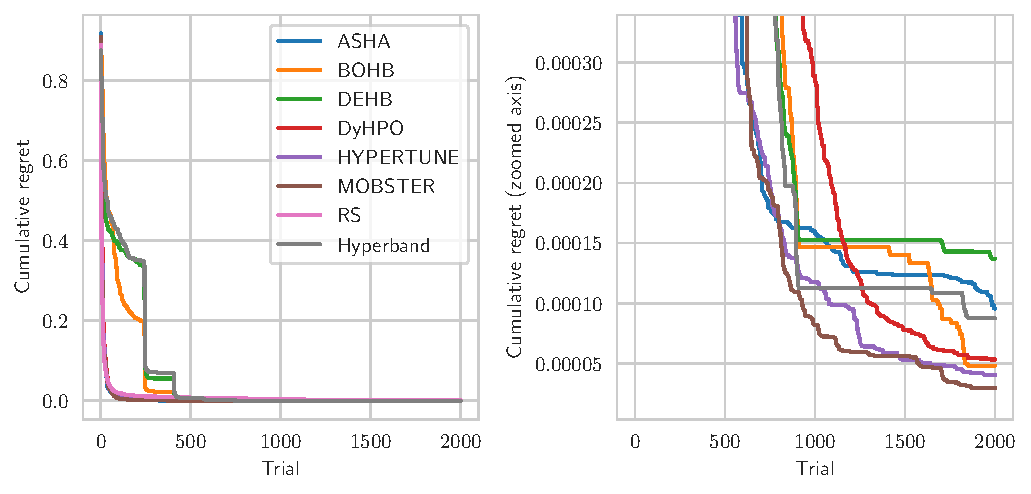
\includegraphics[scale=0.65]{img/tabular_exp/fcnet-naval_plot.pdf}
    \caption{Results of the fcnet-naval experiment.}
    %\label{}
\end{figure}

\begin{figure}[H]
    \centering
    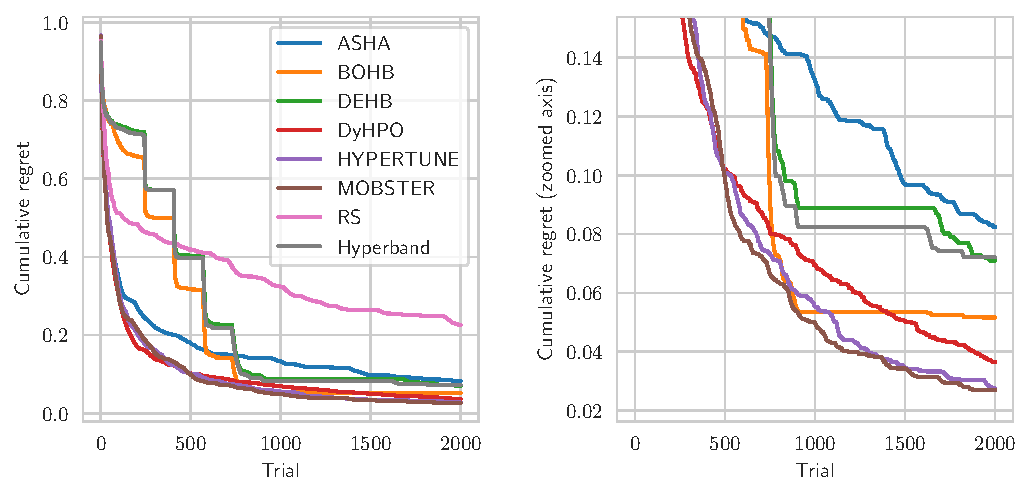
\includegraphics[scale=0.65]{img/tabular_exp/fcnet-protein_plot.pdf}
    \caption{Results of the fcnet-protein experiment.}
    %\label{}
\end{figure}


\begin{figure}[H]
    \centering
    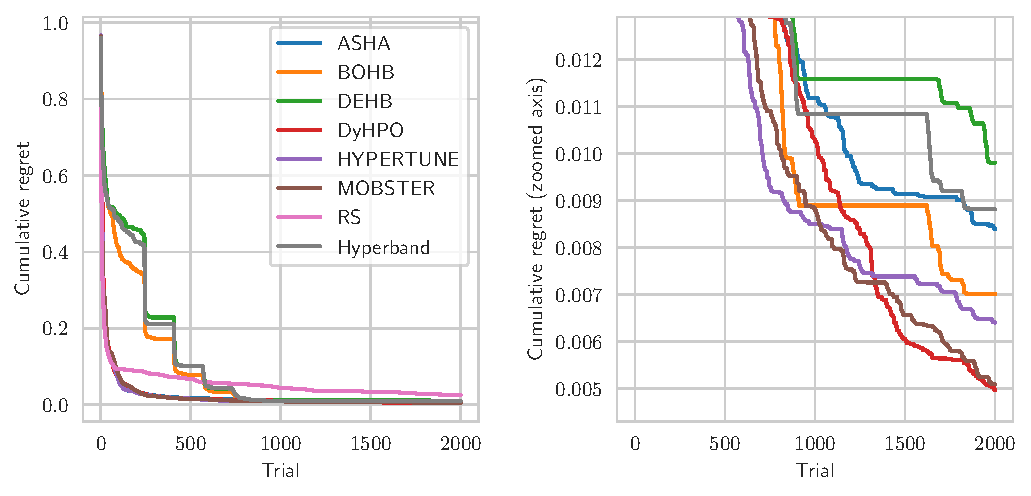
\includegraphics[scale=0.65]{img/tabular_exp/fcnet-parkinsons_plot.pdf}
    \caption{Results of the fcnet-parkinsons experiment.}
    %\label{}
\end{figure}

\begin{figure}[H]
    \centering
    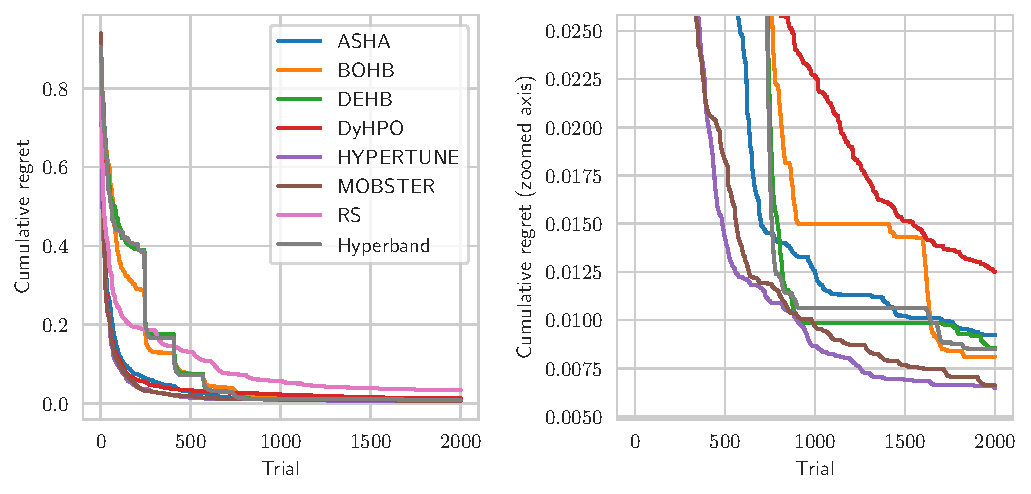
\includegraphics[scale=0.65]{img/tabular_exp/fcnet-slice_plot.pdf}
    \caption{Results of the fcnet-slice experiment.}
    %\label{}
\end{figure}




% NAS-Bench-201: Extending the scope of reproducible neural architecture search. Dong, X. and Yang, Y. 2020.
\begin{figure}[H]
    \centering
    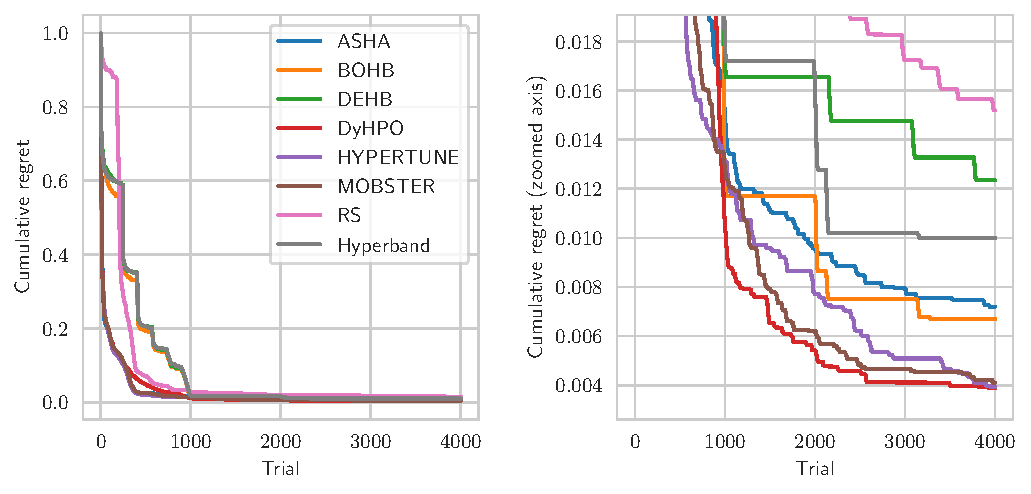
\includegraphics[scale=0.65]{img/tabular_exp/nas201-cifar10_plot.pdf}
    \caption{Results of the nas201-cifar10 experiment.}
    %\label{}
\end{figure}

\begin{figure}[H]
    \centering
    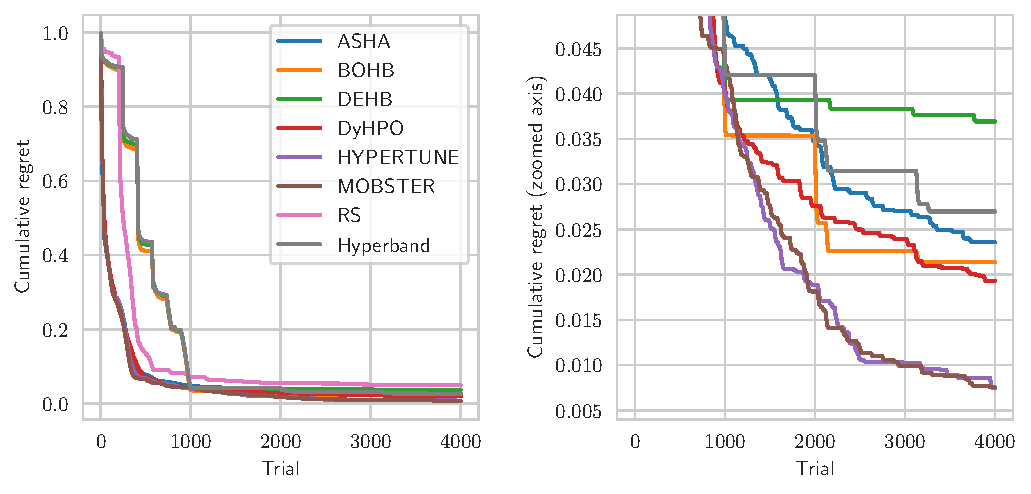
\includegraphics[scale=0.65]{img/tabular_exp/nas201-cifar100_plot.pdf}
    \caption{Results of the nas201-cifar100 experiment.}
    %\label{}
\end{figure}

\begin{figure}[H]
    \centering
    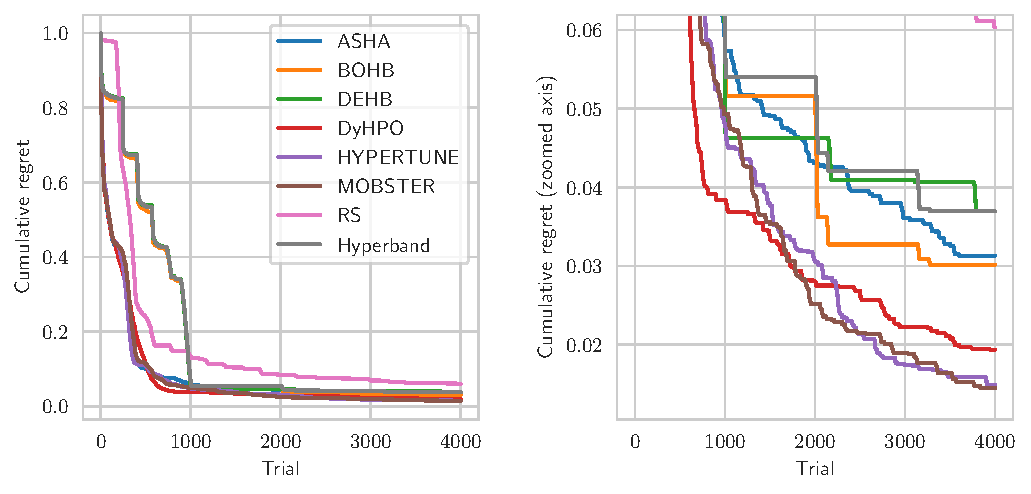
\includegraphics[scale=0.65]{img/tabular_exp/nas201-ImageNet16-120_plot.pdf}
    \caption{Results of the nas201-ImageNet16-120 experiment.}
    %\label{}
\end{figure}

%Reference: Auto-PyTorch: Multi-Fidelity MetaLearning for Efficient and Robust AutoDL. Lucas Zimmer, Marius Lindauer, Frank Hutter. 2020.
\begin{figure}[H]
    \centering
    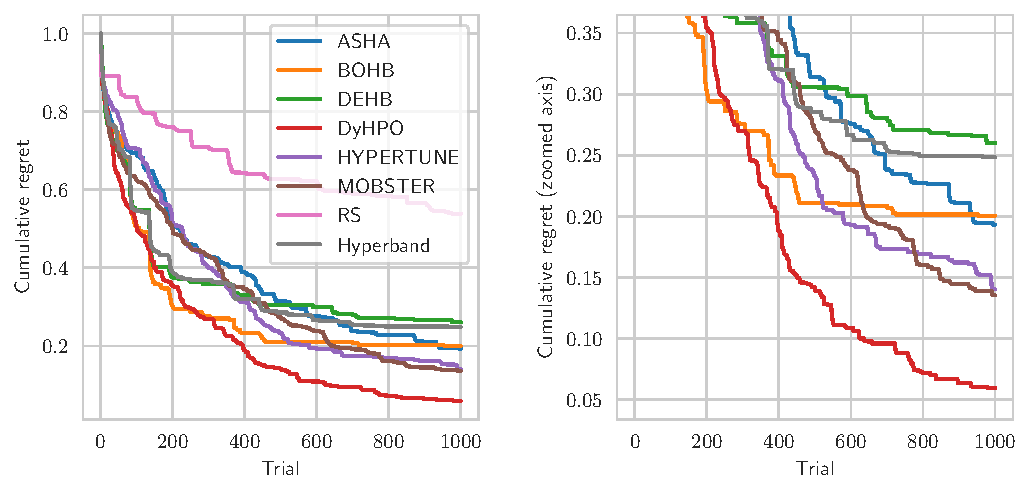
\includegraphics[scale=0.65]{img/tabular_exp/lcbench-airlines_plot.pdf}
    \caption{Results of the lcbench-airlines experiment.}
    %\label{}
\end{figure}

\begin{figure}[H]
    \centering
    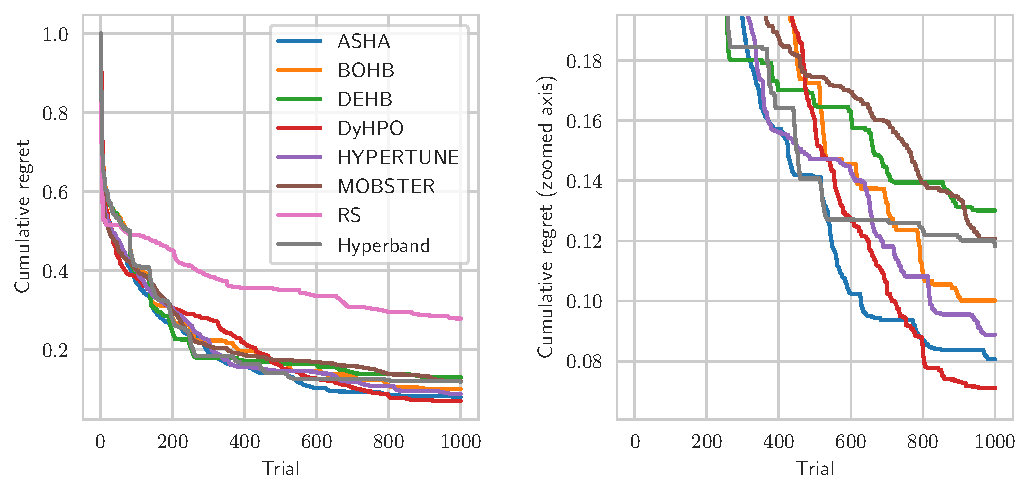
\includegraphics[scale=0.65]{img/tabular_exp/lcbench-albert_plot.pdf}
    \caption{Results of the lcbench-albert experiment.}
    %\label{}
\end{figure}

\begin{figure}[H]
    \centering
    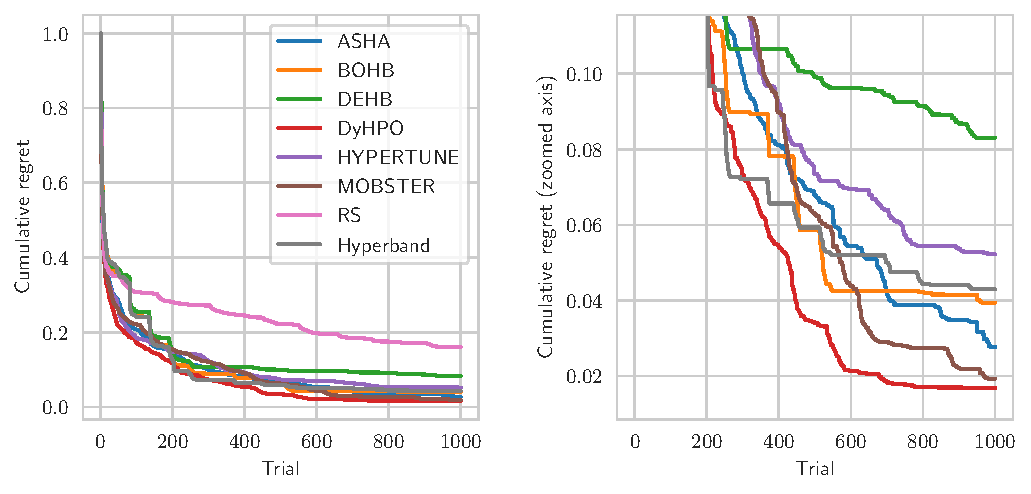
\includegraphics[scale=0.65]{img/tabular_exp/lcbench-Fashion-MNIST_plot.pdf}
    \caption{Results of the lcbench-Fashion-MNIST experiment.}
    %\label{}
\end{figure}

\begin{figure}[H]
    \centering
    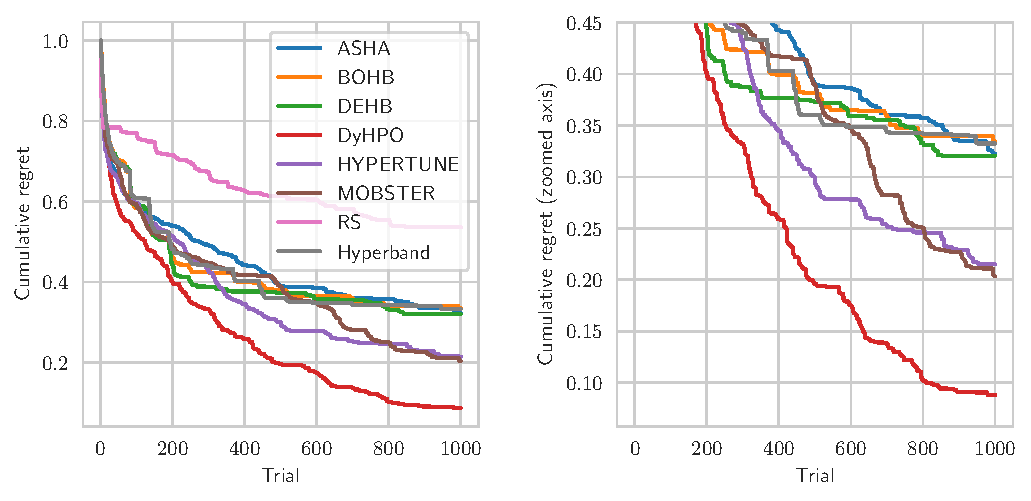
\includegraphics[scale=0.65]{img/tabular_exp/lcbench-covertype_plot.pdf}
    \caption{Results of the lcbench-covertype experiment.}
    %\label{}
\end{figure}

\begin{figure}[H]
    \centering
    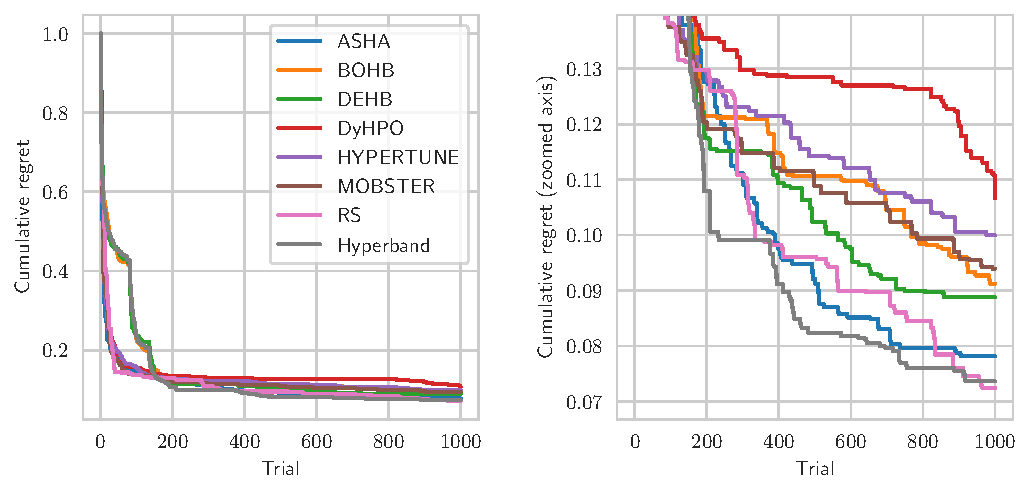
\includegraphics[scale=0.65]{img/tabular_exp/lcbench-christine_plot.pdf}
    \caption{Results of the lcbench-christine experiment.}
    %\label{}
\end{figure}

\begin{figure}[H]
    \centering
    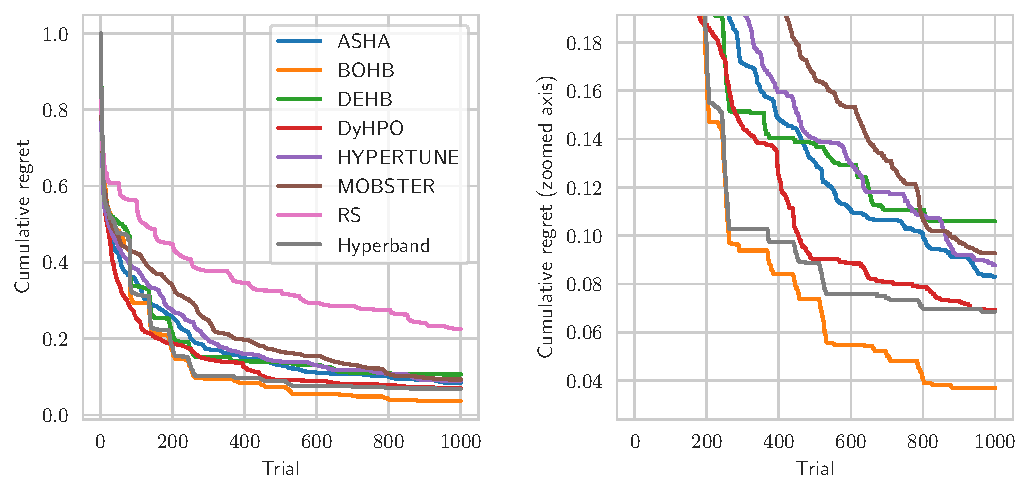
\includegraphics[scale=0.65]{img/tabular_exp/lcbench-higgs_plot.pdf}
    \caption{Results of the lcbench-higgs experiment.}
    %\label{}
\end{figure}

\begin{figure}[H]
    \centering
    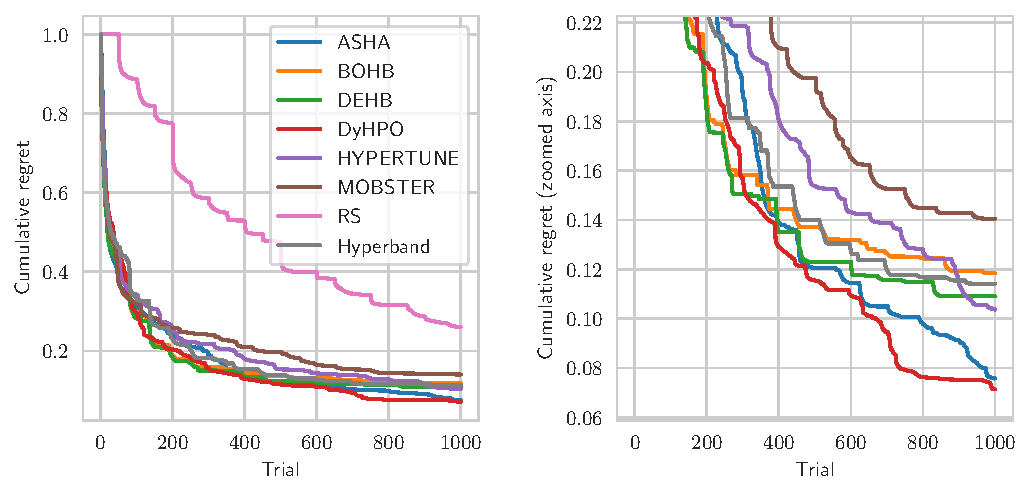
\includegraphics[scale=0.65]{img/tabular_exp/lcbench-dionis_plot.pdf}
    \caption{Results of the lcbench-dionis experiment.}
    %\label{}
\end{figure}

\begin{figure}[H]
    \centering
    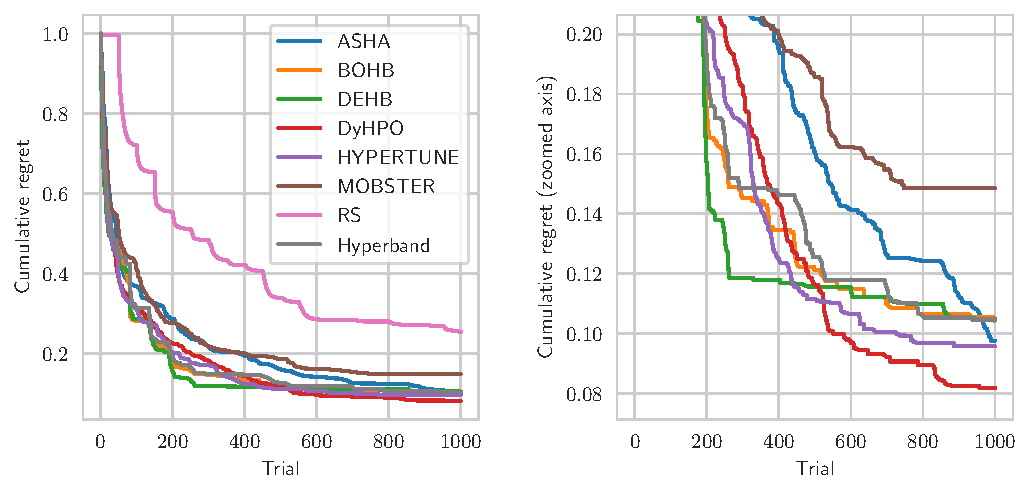
\includegraphics[scale=0.65]{img/tabular_exp/lcbench-helena_plot.pdf}
    \caption{Results of the lcbench-helena experiment.}
    %\label{}
\end{figure}


\section{Real-world}


\begin{figure}[H]
    \centering
    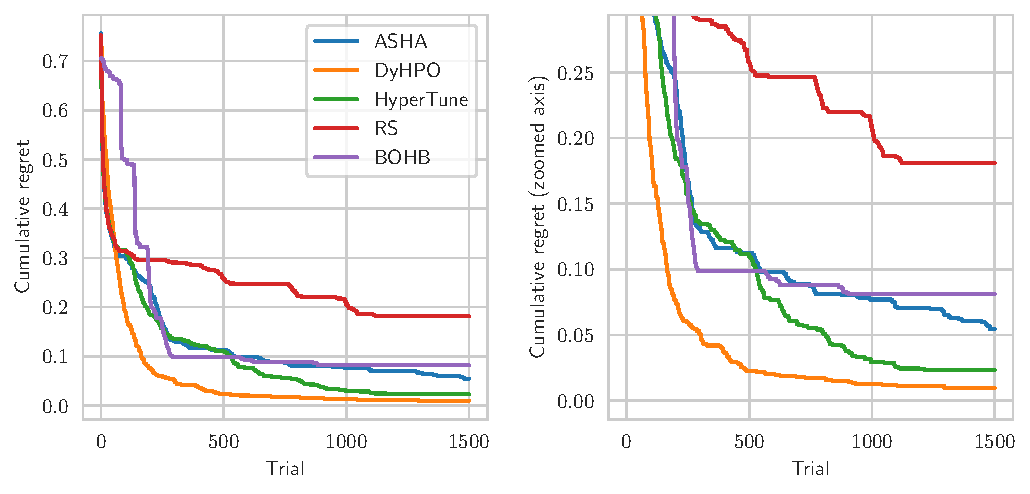
\includegraphics[scale=0.65]{img/real_exp/cifar10_simple_regret_plot.pdf}
    \caption{Results of the cifar10-cnn experiment.}
    \label{fig:cifar10_simple}
\end{figure}

\begin{figure}[H]
    \centering
    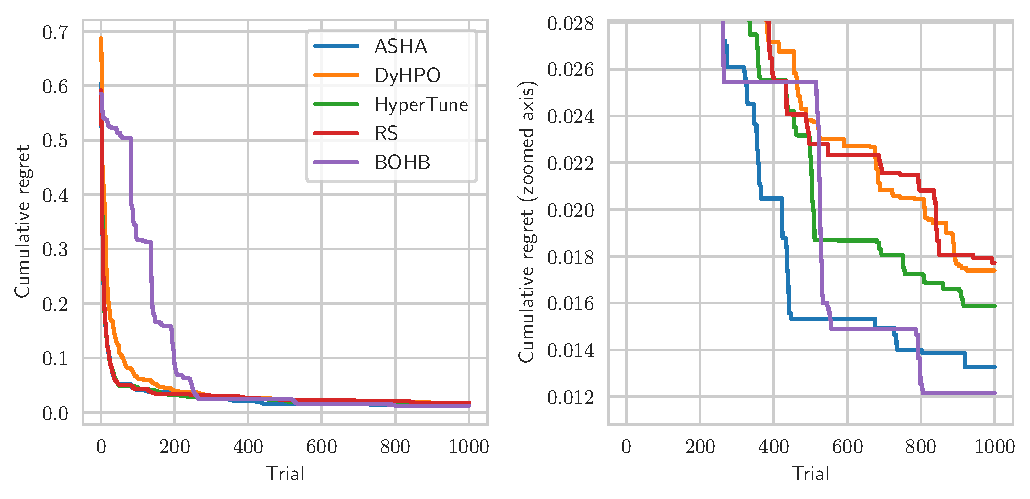
\includegraphics[scale=0.65]{img/real_exp/cifar10_residual_regret_plot.pdf}
    \caption{Results of the cifar10-residual experiment.}
    \label{fig:cifar10_residual}
\end{figure}

\begin{figure}[H]
    \centering
    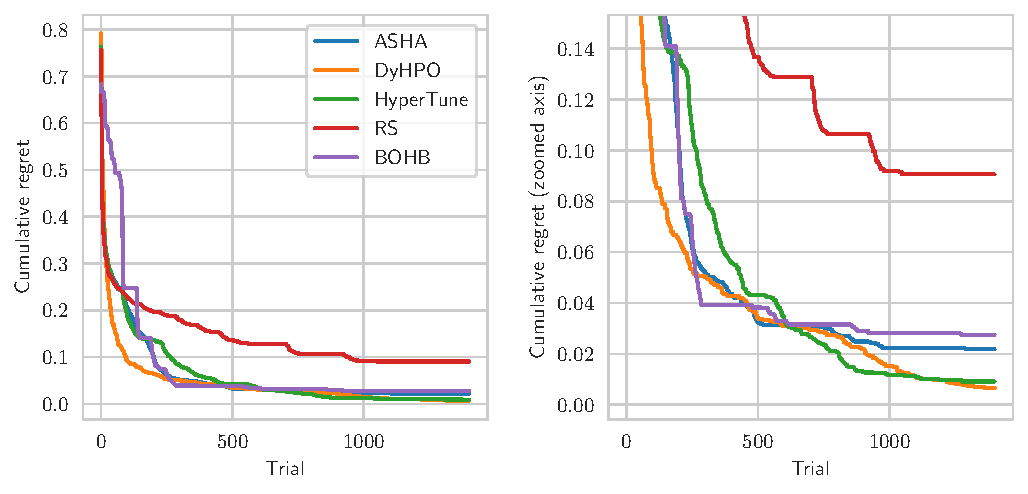
\includegraphics[scale=0.65]{img/real_exp/svhn_simple_regret_plot.pdf}
    \caption{Results of the svhn-cnn experiment.}
    \label{fig:svhn_simple}
\end{figure}

\begin{figure}[H]
    \centering
    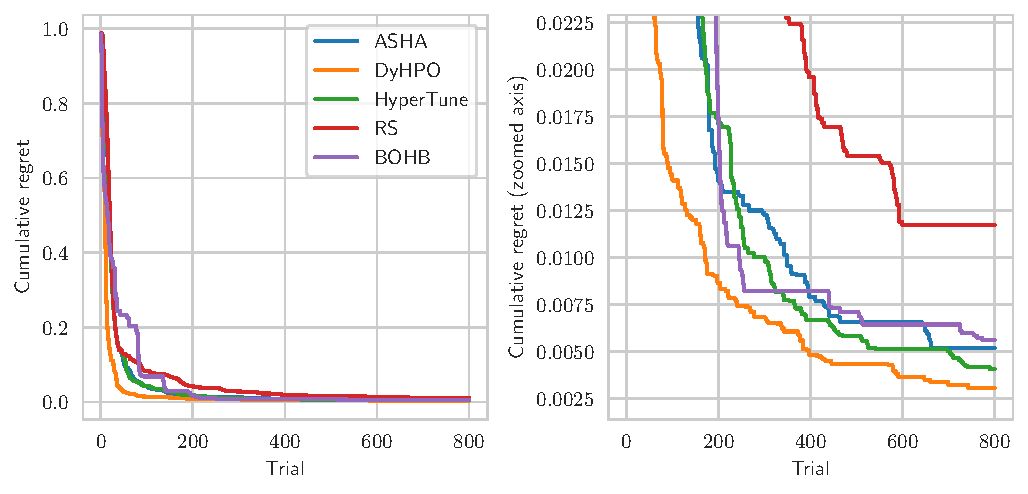
\includegraphics[scale=0.65]{img/real_exp/svhn_residual_regret_plot.pdf}
    \caption{Results of the svhn-residual experiment.}
    \label{fig:svhn_residual}
\end{figure}


\begin{figure}[H]
    \centering
    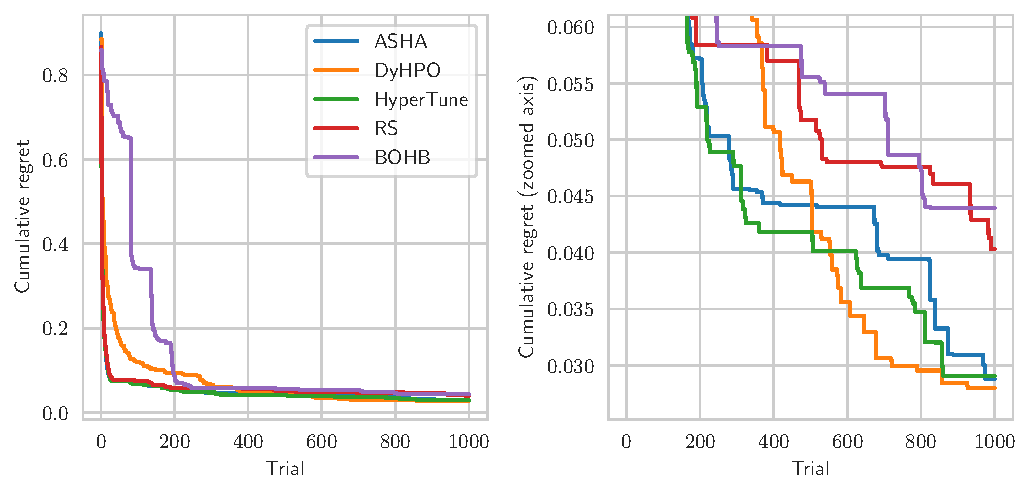
\includegraphics[scale=0.65]{img/real_exp/ptbxl_rnn_regret_plot.pdf}
    \caption{Results of the ptbxl-rnn experiment.}
    \label{fig:ptbxl_rnn}
\end{figure}

\begin{figure}[H]
    \centering
    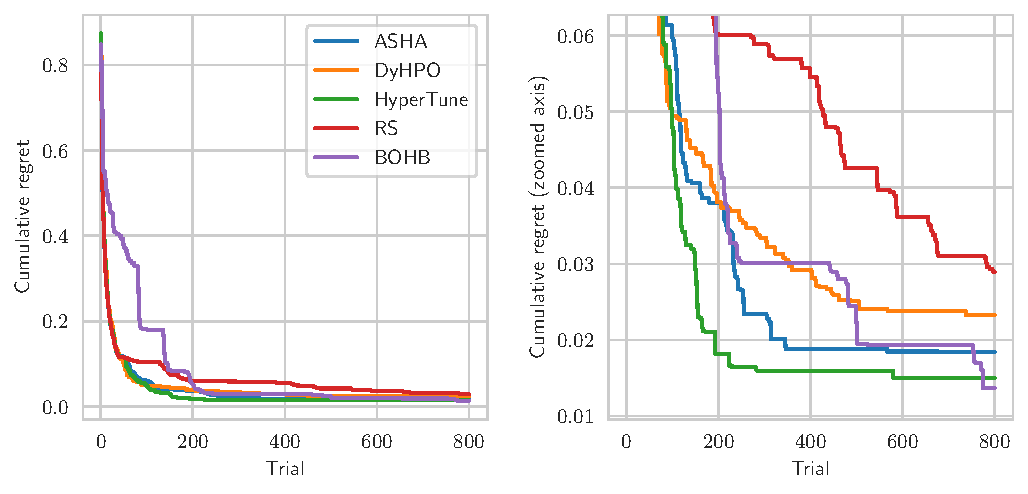
\includegraphics[scale=0.65]{img/real_exp/ptbxl_xResNet1d_regret_plot.pdf}
    \caption{Results of the ptbxl-xResnet1d experiment.}
    \label{fig:ptbxl_xresnet}
\end{figure}

\begin{figure}[H]
    \centering
    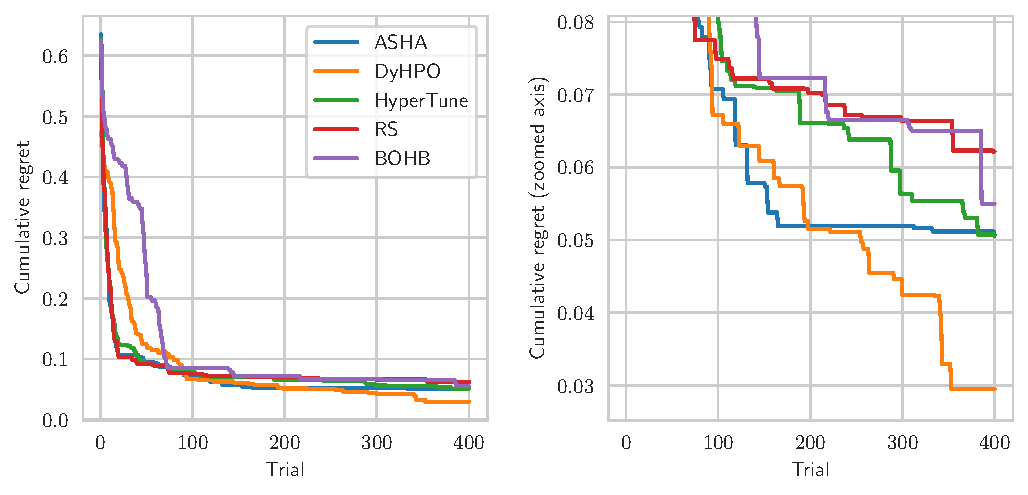
\includegraphics[scale=0.65]{img/real_exp/xray_densenet_regret_plot.pdf}
    \caption{Results of the xray-densenet experiment.}
    \label{fig:xray_densenet}
\end{figure}


% if your attachments are complicated, describe them in a separate appendix
%\include{attachments}

%\openright
\end{document}
